% Drawing 154/04-1 -- folder 154, batch 04, archive page 64 (PDF page 65).
% Transcription: figures : deux grands disques côte à côte. À gauche, $\Delta_{D'}$, au bord vert foncé (légende $D'$) : deux pseudo-droites orange qui se croisent en $s$ juste au-dessous du bord, en haut, où un segment épais noir marque l'arc $a$ et un arc pointillé l'arc $a'$ ; un petit cercle vert clair y figure le recollement ; une croix orange (point double) près du bord. À droite, $\Delta_D$, au bord vert clair (légende $D$, $\Delta_D$) : deux pseudo-droites orange, un segment épais noir en bas (l'arc $b$, près de $s$) et une rangée de points noirs en haut (l'arc $b'$), une croix orange
% Kind: two disks Delta_{D'} and Delta_D with two pseudolines. Method 2 (schematic redraw from the facsimile). Status: ok.
% Notes: Two large disks side by side. Left, Delta_{D'}, dark green rim (legend D'): two orange pseudolines forming a long spindle, crossing at s just under the rim at the top, where a thick black segment marks the arc a and a dotted arc the arc a' (the dashed inner arcs near top and bottom); small light green circles at the top and the bottom figure the gluing; an orange cross (double point) near the rim. Right, Delta_D, light green rim (legend D, Delta_D): two orange pseudolines, a thick black segment at the bottom (the arc b, near s) and a row of black points at the top (the arc b'), an orange cross. Read from the page view; labels a, a', b, b' placed approximately.
% Coordinates: 1 unit = 1 mm = 1/100 of the crop width (bbox in page fractions: [0.139, 0.079, 0.687, 0.278]).
% Redrawn by Claude (claude-opus-5-5), issue #73, 2026-11-07; not checked by a human; not compiled (no TeX in the session).
% Rights: reproduces part of the work -- behind RENDER_TRANSCRIPTS, never published by itself.
\documentclass[tikz,border=3pt]{standalone}
\usepackage{amsmath,amssymb}
\usetikzlibrary{patterns,arrows.meta}
\tikzset{Or/.style={orange!90!black}, Ye/.style={yellow!80!orange}, Lg/.style={green!60!black!70}, Dg/.style={green!45!black}, Br/.style={brown!80!black}, Rd/.style={red!85!black}, Bl/.style={blue!70!black}, Gy/.style={black!40}, pencil/.style={black!45}, struck/.style={black!35}, mark/.style={circle,draw,inner sep=1.3pt}, pt/.style={circle,fill,inner sep=0.9pt}, opt/.style={circle,draw,fill=white,inner sep=1.1pt}}
\begin{document}
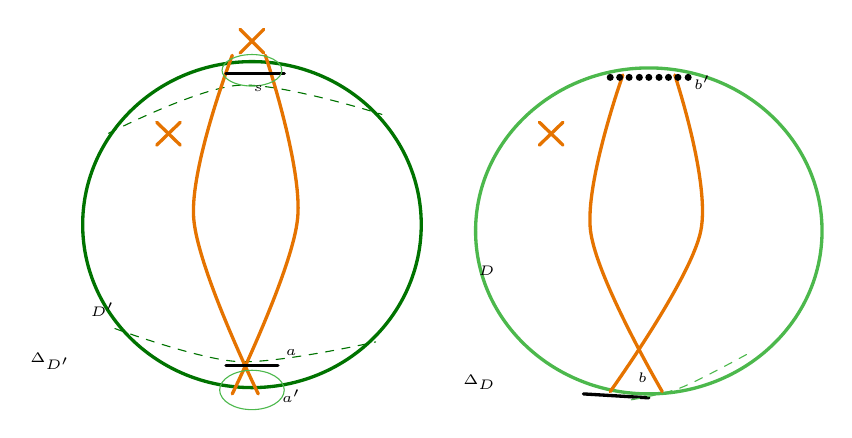
\begin{tikzpicture}[x=1mm,y=1mm,line cap=round,line join=round,font=\scriptsize]
\draw[Dg,very thick] (28.1,-25.6) ellipse[x radius=21.5, y radius=20.7];
\draw[Dg,dashed] plot[smooth, tension=0.55] coordinates {(9.9,-14) (26.4,-7.9) (44.6,-11.6)};
\draw[Dg,dashed] plot[smooth, tension=0.55] coordinates {(10.7,-38.8) (26.4,-43) (43.8,-40.5)};
\draw[Or,very thick] plot[smooth, tension=0.55] coordinates {(25.6,-4.1) (20.7,-24.8) (28.9,-47.1)};
\draw[Or,very thick] plot[smooth, tension=0.55] coordinates {(29.8,-4.1) (33.9,-24.8) (25.6,-47.1)};
\draw[very thick] (24.8,-6.4) -- (32.2,-6.4);
\draw[very thick] (24.8,-43.5) -- (31.4,-43.5);
\draw[Lg] (28.1,-6) ellipse[x radius=3.8, y radius=2];
\draw[Lg] (28.1,-46.6) ellipse[x radius=4.1, y radius=2.5];
\draw[Or,very thick] (26.6,-0.8) -- (29.6,-3.8);
\draw[Or,very thick] (26.6,-3.8) -- (29.6,-0.8);
\draw[Or,very thick] (16,-12.6) -- (19,-15.5);
\draw[Or,very thick] (16,-15.5) -- (19,-12.6);
\node[inner sep=1pt] at (9.1,-36.4) {\tiny $D'$};
\node[inner sep=1pt] at (2.5,-43) {\tiny $\Delta_{D'}$};
\node[inner sep=1pt] at (33.1,-41.8) {\tiny $a$};
\node[inner sep=1pt] at (33.1,-47.4) {\tiny $a'$};
\node[inner sep=1pt] at (28.9,-8.3) {\tiny $s$};
\draw[Lg,very thick] (78.5,-26.4) ellipse[x radius=22, y radius=20.7];
\draw[Or,very thick] plot[smooth, tension=0.55] coordinates {(75.2,-6.6) (71.1,-26.4) (80.2,-46.8)};
\draw[Or,very thick] plot[smooth, tension=0.55] coordinates {(81.8,-6.6) (85.1,-26.4) (73.6,-46.8)};
\node[pt] at (73.6,-6.9) {};
\node[pt] at (74.8,-6.9) {};
\node[pt] at (76,-6.9) {};
\node[pt] at (77.3,-6.9) {};
\node[pt] at (78.5,-6.9) {};
\node[pt] at (79.8,-6.9) {};
\node[pt] at (81,-6.9) {};
\node[pt] at (82.2,-6.9) {};
\node[pt] at (83.5,-6.9) {};
\node[inner sep=1pt] at (85.3,-7.6) {\tiny $b'$};
\draw[very thick] (70.2,-47.1) -- (78.5,-47.6);
\node[inner sep=1pt] at (77.7,-45) {\tiny $b$};
\draw[Or,very thick] (64.6,-12.6) -- (67.6,-15.5);
\draw[Or,very thick] (64.6,-15.5) -- (67.6,-12.6);
\node[inner sep=1pt] at (57.9,-31.4) {\tiny $D$};
\node[inner sep=1pt] at (57,-45.6) {\tiny $\Delta_D$};
\draw[Lg,dashed] plot[smooth, tension=0.55] coordinates {(90.9,-42.1) (82.6,-46.3) (76,-47.9)};
\end{tikzpicture}
\end{document}
